\section[Concentration Profiles and Principal Component Analysis]{Temporally Ordering Pre-Aligned Concentration Profiles Using~Principal~Component~Analysis}

\begin{frame}{Principal Component Analysis for Ordering Data}

    \begin{columns}[T]
        \begin{column}{0.3 \textwidth}
            \includegraphics[width=0.8\textwidth]{../Stas_data/group_meeting_5Feb2013/example1_all}

            {\scriptsize This data is similar to the {\em Drosphila} data; it is clearly ordered in time \par}
        \end{column}

        \begin{column}{0.3 \textwidth}
            \includegraphics[width=0.8\textwidth]{../Stas_data/group_meeting_5Feb2013/example1_coarse}

            {\scriptsize We can look at a ``coarsened'' representation of the data with only three spatial components \par}
        \end{column}

        \begin{column}{0.3 \textwidth}
            \includegraphics[width=0.8\textwidth]{../Stas_data/group_meeting_5Feb2013/example1_embedding}

            {\scriptsize If we plot the three-dimensional data and color them in time, we see they fall on a line and are correlated along this line in time \par}
        \end{column}
    \end{columns}
    %\vspace{0.1 in}

	\begin{columns}
	\begin{column}{0.7\textwidth}
	\begin{itemize}
	{\small   
   \item If we embedded the original (high-dimensional) data, the data would fall on a line in high-dimensional space

   \item We assume that the data is ordered in time when projected along this line
   
   \item We would like an automatic way to find this line in higher dimensions
      
  \item Principal Component Analysis (PCA) \footnotemark finds this line by calculating the direction(s) of maximum variance %in a data set
  \par}
  \end{itemize}
  \end{column}
  \begin{column}{0.25\textwidth}
  \begin{block}{{\small PCA Algorithm}}
 {\footnotesize
  	Calculate covaraince matrix
  	$$C =X^T X$$	
  	Compute eigenvectors and eignevalues
  	$$C V = V \Lambda$$
  	$V$ are the principal components
  %\end{block}
  \par}
  \end{block}
  \end{column}
  \end{columns}
  
  \footcitetext{shlens2005tutorial}
\end{frame}

%\begin{frame}{PCA: Covariance Matrix}
%  \begin{itemize}
%  \item We have $n$ {\bf data points}, each in $d$ dimensions, denoted $x_1, x_2, \dots, x_n \in \mathbb{R}^d$, where $x_{i,j}$ denotes the $j^{th}$ component of data point $i$
%  \item We first define the {\bf mean-centered} data points $\hat{x}_i$ as $$\hat{x}_{i,j} = x_{i,j} - \frac{1}{n} \sum_{i=1}^{n} x_{i,j}$$
%  \item Let $X \in \mathbb{R}^{n \times d}$ denote the data matrix, where the $i^{th}$ row of $X$ contains $\hat{x}_i$
%  \item The {\bf covariance matrix} $R \in \mathbb{R}^{d \times d}$ can be estimated as $$R = \frac{1}{n-1} X^T X$$
%  \end{itemize}
%\end{frame}
%
%\begin{frame}{PCA: Eigendecomposition}
%\begin{columns}
%\begin{column}{0.7\textwidth}
%  \begin{itemize}
%    \item We then compute the {\bf eigenvectors} $v_1, v_2, \dots, v_d$ and {\bf eigenvalues} $\lambda_1, \lambda_2, \dots, \lambda_d$ of $R$ (all eigenvectors are normalized to 1)
%    \item By construction, $R$ is symmetric and positive semi-definite and is therefore guaranteed to have real non-negative eigenvalues and orthogonal real eigenvectors
%    \item We {\bf order} the eigenvector/eigenvalue pairs such that $\lambda_1 \ge \lambda_2 \ge \dots \ge \lambda_d$
%    \item $v_1, v_2, \dots, v_d$ are called the {\bf principal components}, and $\lambda_j$ measures the {\bf variance} captured by principal component $j$
%  \end{itemize}
%  \end{column}
%
%  \begin{column}{0.3\textwidth}
%        \includegraphics[width=\textwidth]{../Stas_data/group_meeting_5Feb2013/PCA_spectrum1.jpg}\\
%        {\tiny The PCA eigenvalue spectrum; each eigenvalue measures the energy captured by the corresponding eigenvector \par}
%
%        \vspace{0.3 in}
%
%        \includegraphics[width=\textwidth]{../Stas_data/group_meeting_5Feb2013/PCA_mode1.jpg}\\
%        {\tiny The first principal component \par}
%
%  \end{column}
%  \end{columns}
%\end{frame}
%
%\begin{frame}{PCA: Ordering and Projections}
%    \begin{itemize}
%        \item We can calculate the projection of data point $i$ onto principal component $j$ as $a_{i,j} = \langle \hat{x}_i, v_j \rangle = \sum_{k=1}^{d} \hat{x}_{i,k} v_{j,k}$
%        \item $a_{i,j}$ can be viewed as a measure of how much principal component $j$ is represented in data point $i$
%        \item We can order the data by $a_{i,1}$
%        \item Each principal component defines an important ``direction'' in our data; we can compare data sets by comparing their principal components
%    \end{itemize}
%
%    \centering
%    \includegraphics[height=0.3\textheight]{../Stas_data/group_meeting_5Feb2013/data1_scrambled.jpg}
%    \includegraphics[height=0.3\textheight]{../Stas_data/group_meeting_5Feb2013/coeff_scrambled.jpg}\\
%    {\Tiny The scrambled data (left) and the projection coefficient for each data point onto the first principal component (right).\\
%    We will sort the data by the values of the projection coefficients. \par}
%
%\end{frame}

\begin{frame}{Ordering {\em Drosophila} Data using PCA}

	\centering
	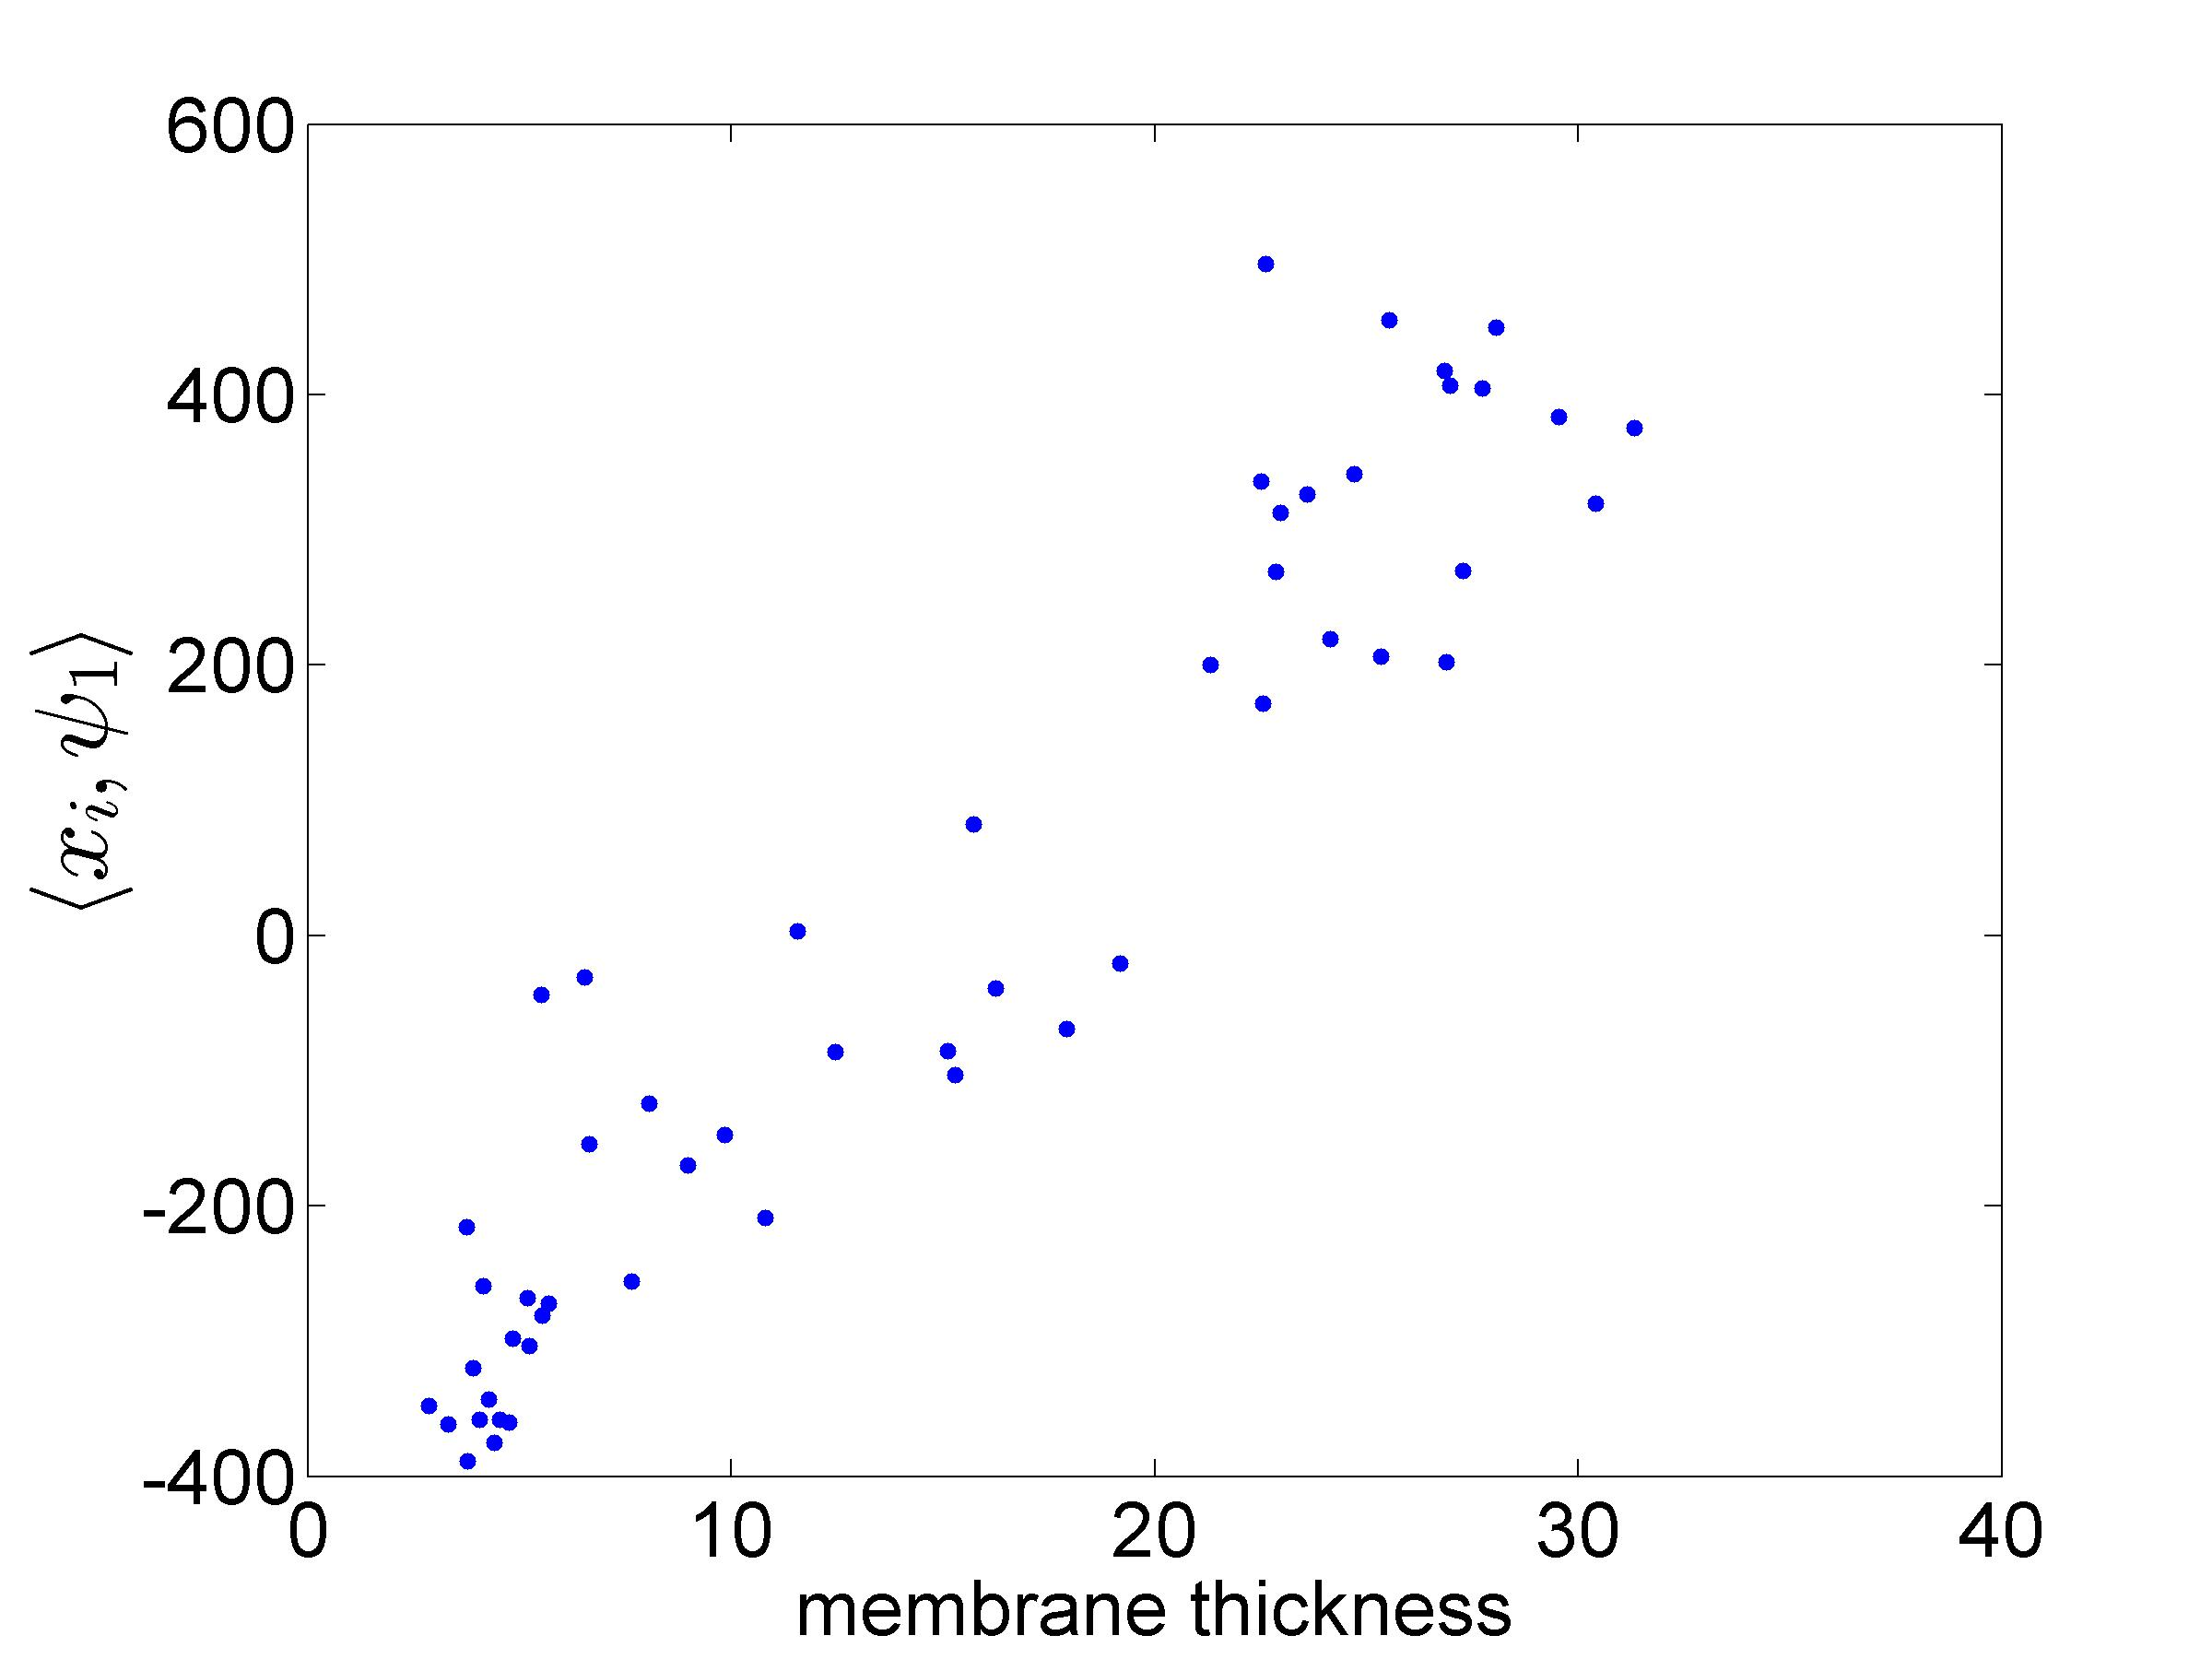
\includegraphics[width=0.3\textwidth]{PCA_time_corr}	
  
  \centering
  \begin{tikzpicture}
  	\node (unordered) {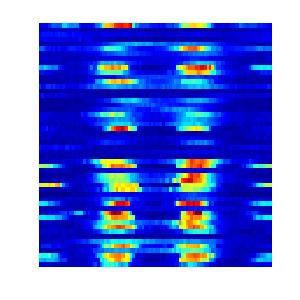
\includegraphics[width=0.3\textwidth]{data_unordered}};
  	\node[right of=unordered, node distance=0.5\textwidth] (ordered) {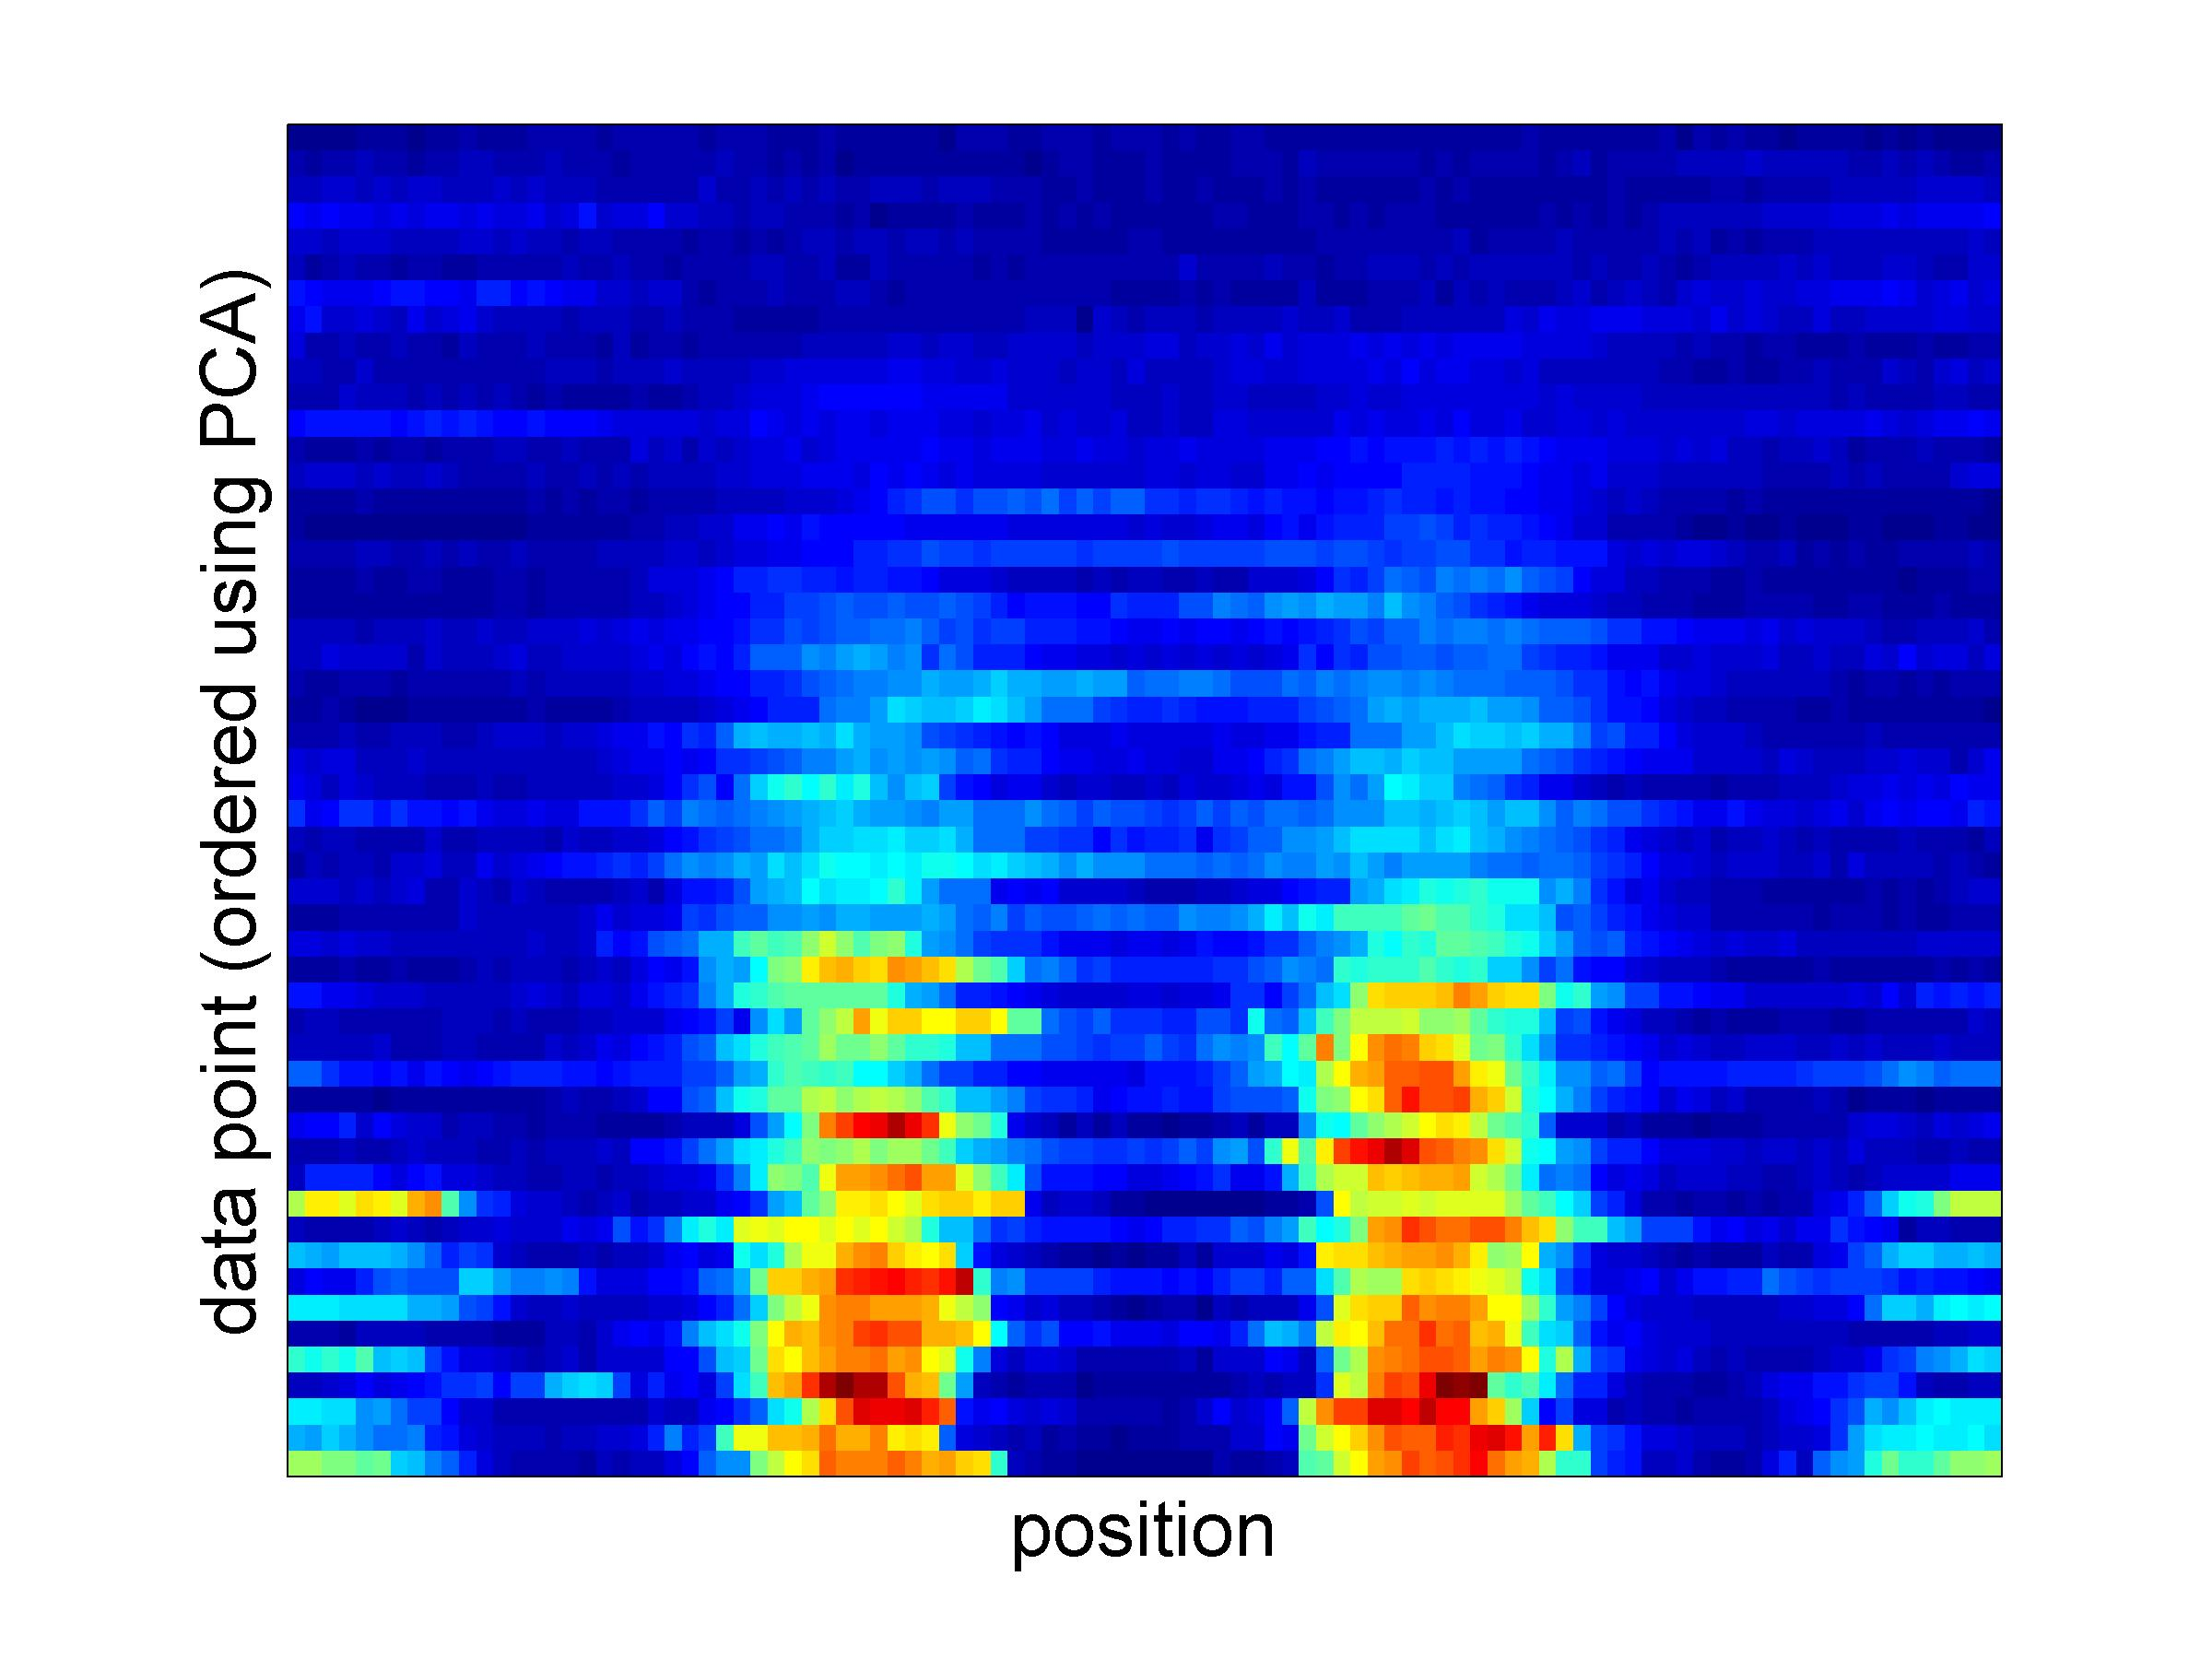
\includegraphics[width=0.3\textwidth]{data_ordered_PCA}};
    \draw [->] (unordered.east) -- (ordered.west);    
  \end{tikzpicture}
  
	
	
\end{frame}


\begin{frame}{Some Problems with PCA}
    \centering
    \begin{tikzpicture}
    	\node[anchor=south west] (PCA_fig) {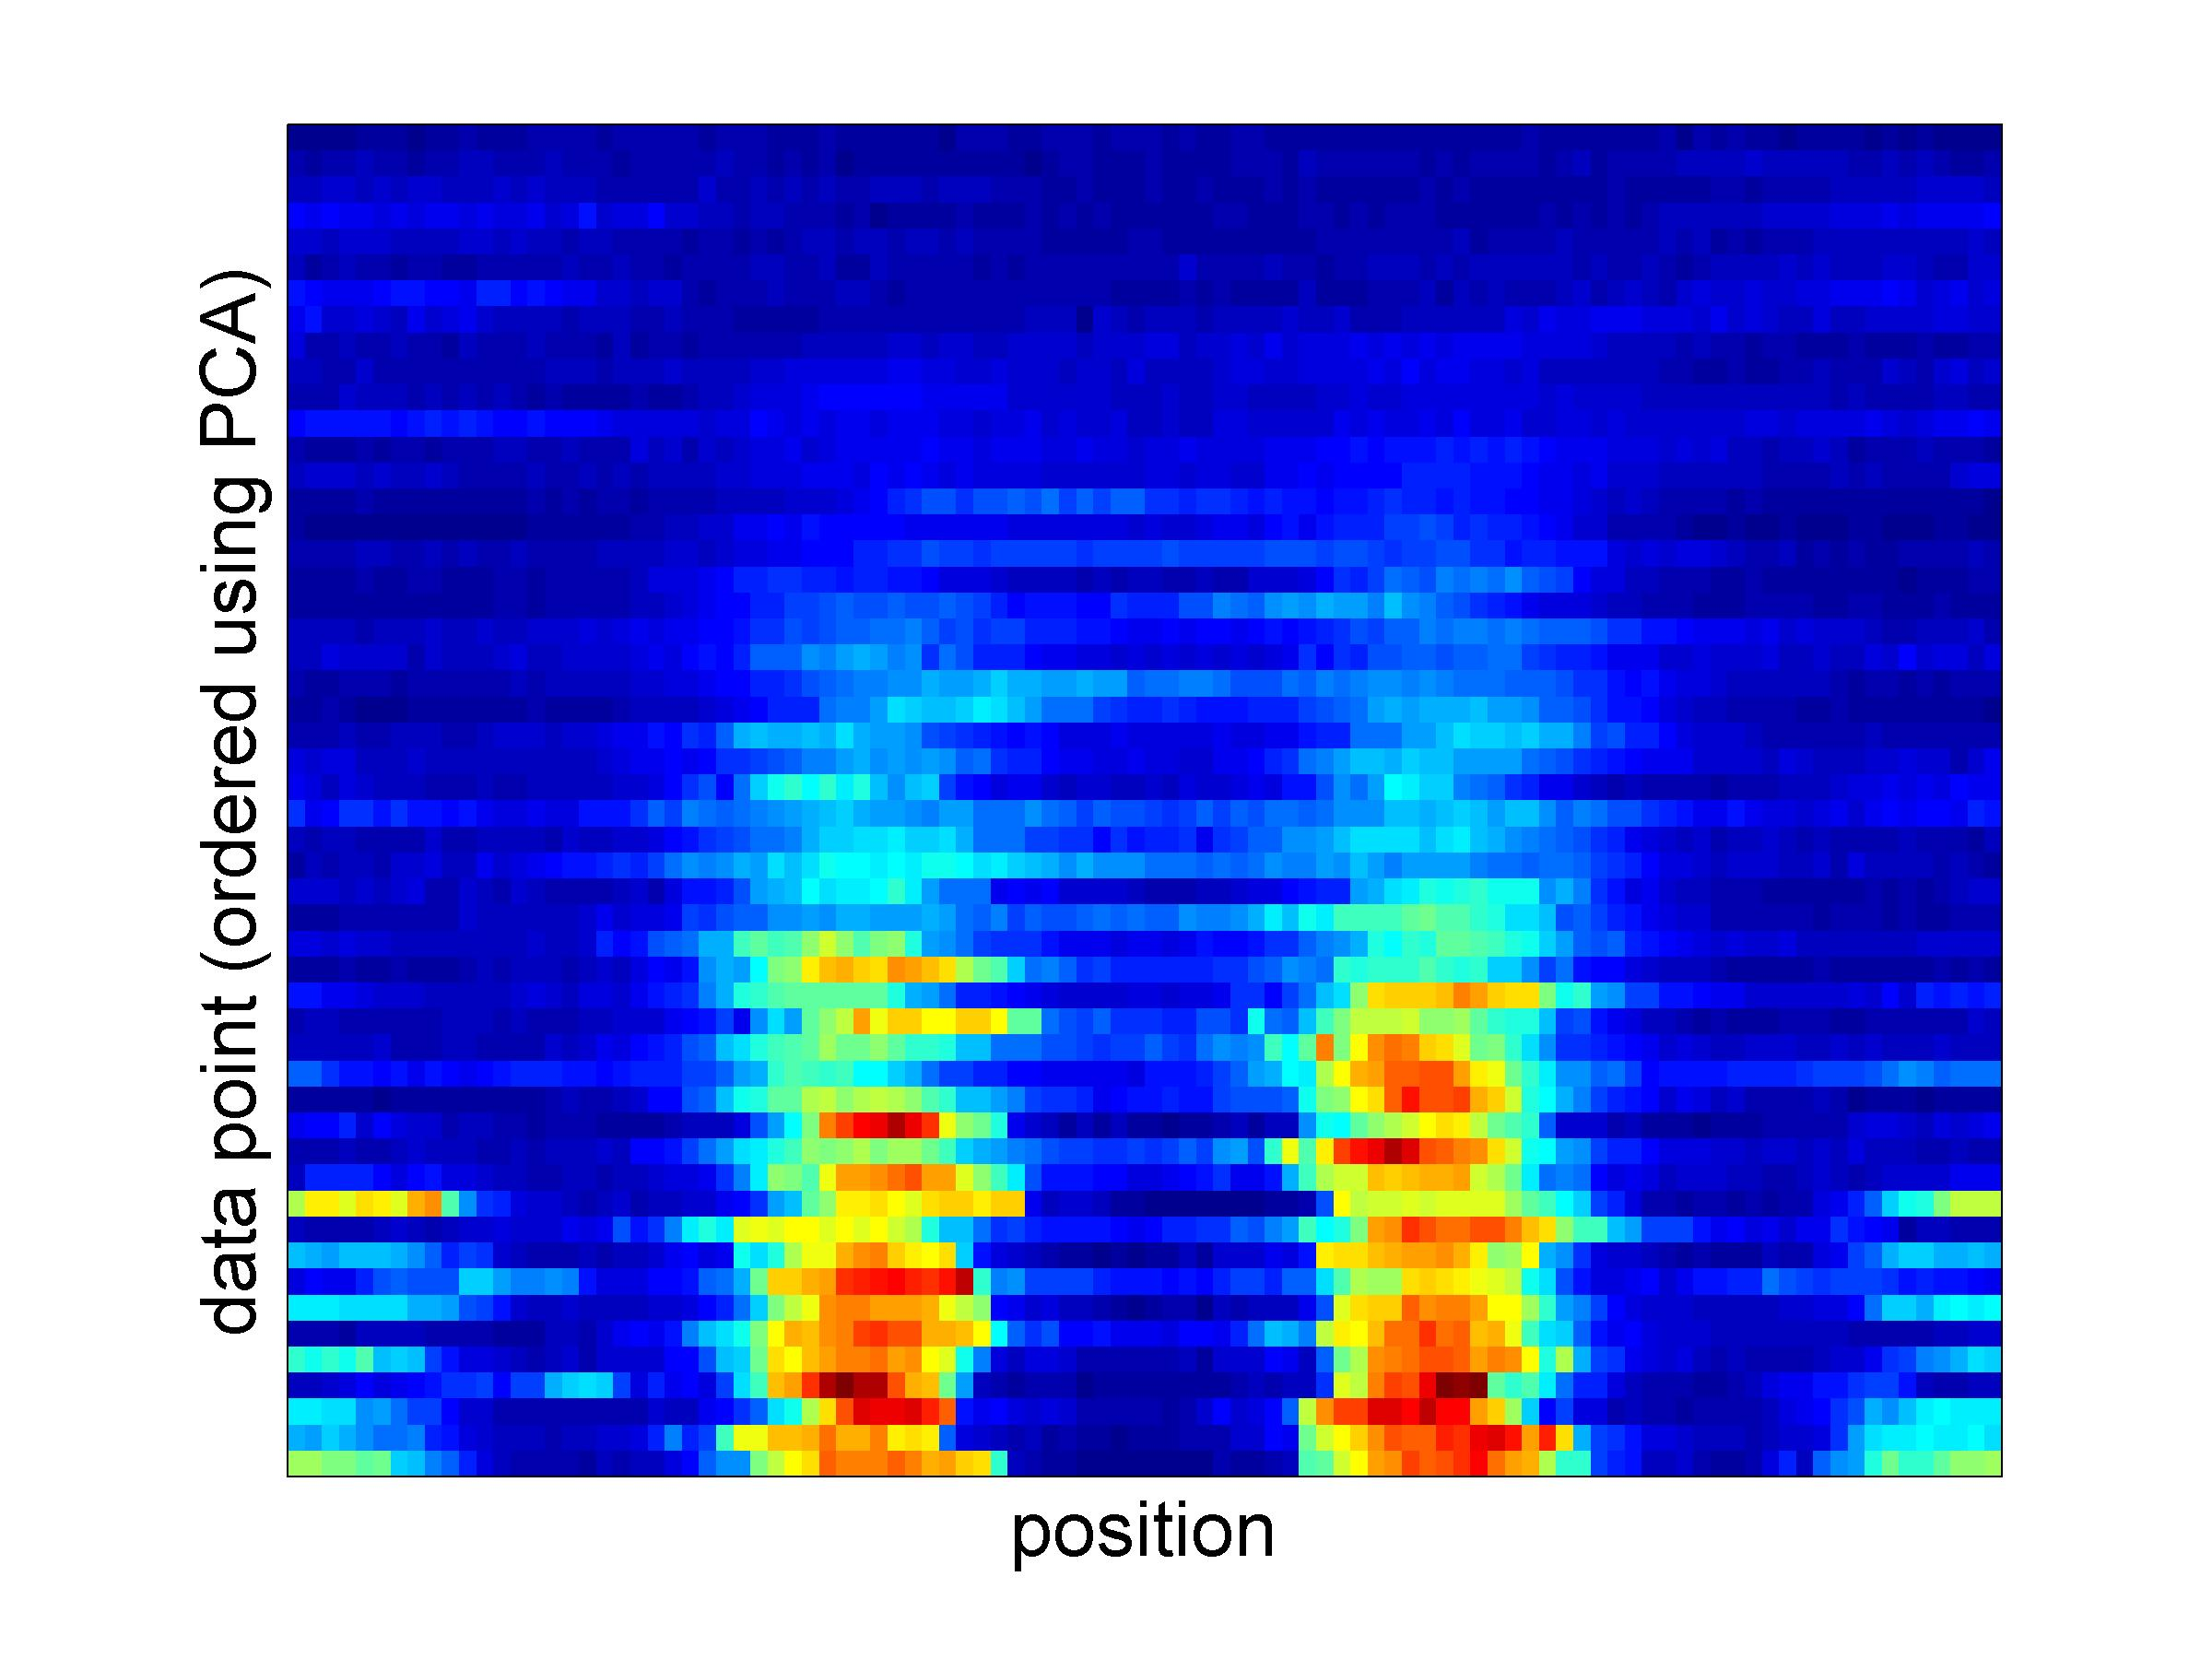
\includegraphics[width=0.5\textwidth]{data_ordered_PCA}};
    	\begin{scope}[x={(PCA_fig.south east)},y={(PCA_fig.north west)}]
    	%\draw[help lines,xstep=.05,ystep=.05] (0,0) grid (1,1);
    	\draw[rounded corners=1mm, line width=0.5mm, red] (0.13,0.13) rectangle (0.22,0.3);
    	\draw[rounded corners=1mm, line width=0.5mm, red] (0.81,0.13) rectangle (0.9,0.3);
    	\end{scope}
    	\node[anchor=south west, right of=PCA_fig, node distance=0.5\textwidth] (DMAPS_fig) {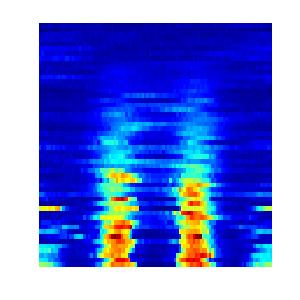
\includegraphics[width=0.5\textwidth]{data_ordered_DMAPS}};
    	\begin{scope}[shift={(DMAPS_fig.south west)},x={(DMAPS_fig.south east)},y={(DMAPS_fig.north west)}]
    	\draw[rounded corners=1mm, line width=0.5mm, red] (0.13,0.13) rectangle (0.22,0.3);
    	\draw[rounded corners=1mm, line width=0.5mm, red] (0.81,0.13) rectangle (0.9,0.3);
    	\end{scope}
    \end{tikzpicture}
    
   
    The ordering of the large central peaks is comparable.\\
    However, the outer peaks are grouped together in the right picture \\ (we could view this as ``better'').

\end{frame}

\begin{frame}{Nonlinear Orderings of Data}

	\centering
	Below are the first two projection coefficients for the data \\
	(each point corresponds to a data point/concentration profile).
	
    \centering
    \only<1>{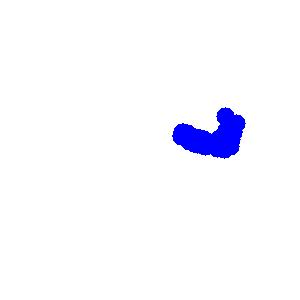
\includegraphics[width=0.6\textwidth]{coeff_12_new}}
    \only<2>{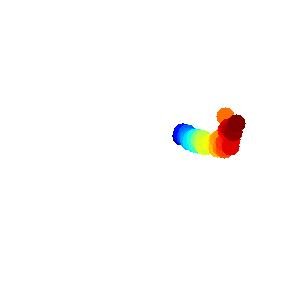
\includegraphics[width=0.6\textwidth]{coeff_12_colored}}
	
    We only use the first coefficient in the PCA ordering.
	\pause
	
	The ordering of the data produced with this coloring would perhaps be better. \\
    PCA cannot detect this ordering because it is nonlinear.
    
\end{frame}

\begin{frame}{Diffusion Maps (DMAPS) for Dimensionality Reduction}
\centering
Unlike PCA, diffusion maps \footnote{ \tiny Coifman {\em et al}, PNAS, 2005.} is a {\em nonlinear} dimensionality reduction technique

	\begin{columns}
	\begin{column}{0.4\textwidth}
		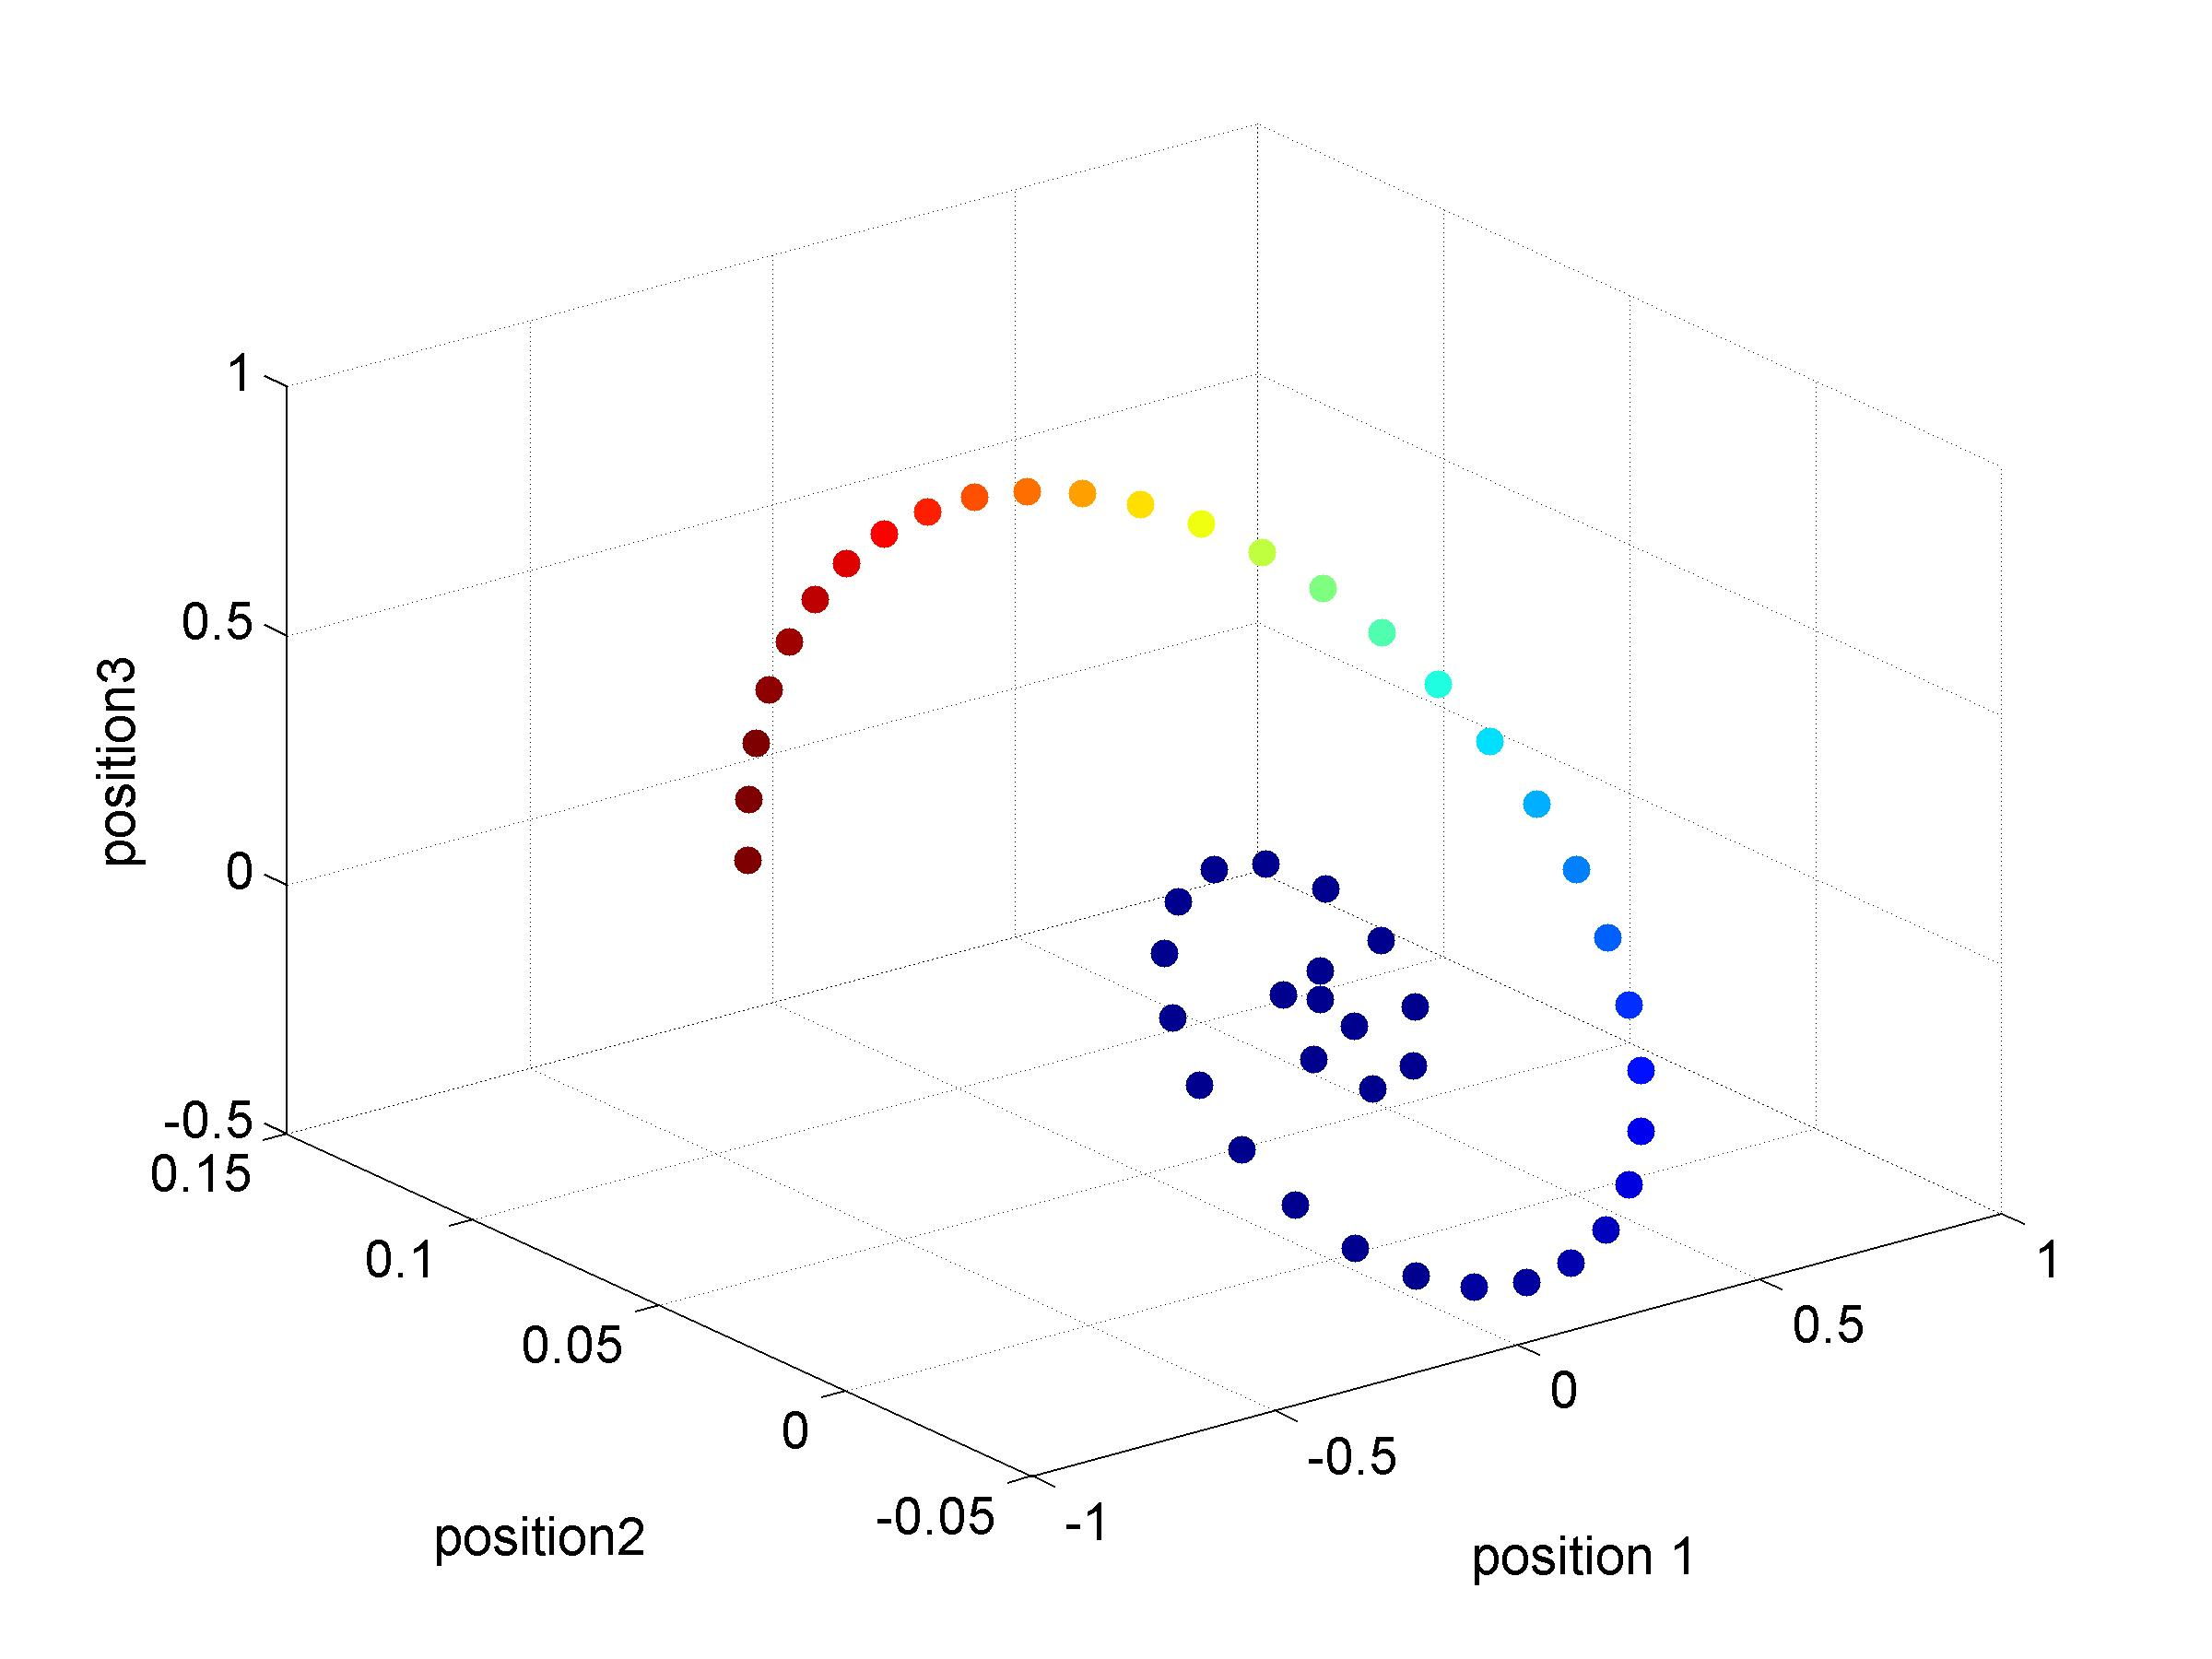
\includegraphics[width=\textwidth]{../Stas_data/group_meeting_5Feb2013/dmaps_spiral.jpg}
	\end{column}
	\begin{column}{0.5\textwidth}
	\begin{block}{DMAPS Algorithm}
		{\scriptsize 
		Calculate weight matrix $W$ with
		$$W_{ij} = exp\left( -\frac{d^2(x_i, x_j)}{\epsilon} \right)$$
		Calculate diagonal matrix $D$ with $D_{ii} = \sum_j W_{ij}$
		
		The embedding coordinates are given by the {\bf top~eigenvectors} of $D^{-1}W$
		\par}
	\end{block}
	\end{column}
	\end{columns}
%On the left you see data that has been ordered and colored using PCA.
%On the right you see data that has been ordered and colored using DMAPS.

\vspace{0.2in}

The spiral has been colored using DMAPS.

PCA would not be able to order the data on the right ``correctly'', \\since the curve is one-dimensional, but non-linear.

\end{frame}

\begin{frame}{Using DMAPS to Order Concentration Profiles}

	
	\centering
	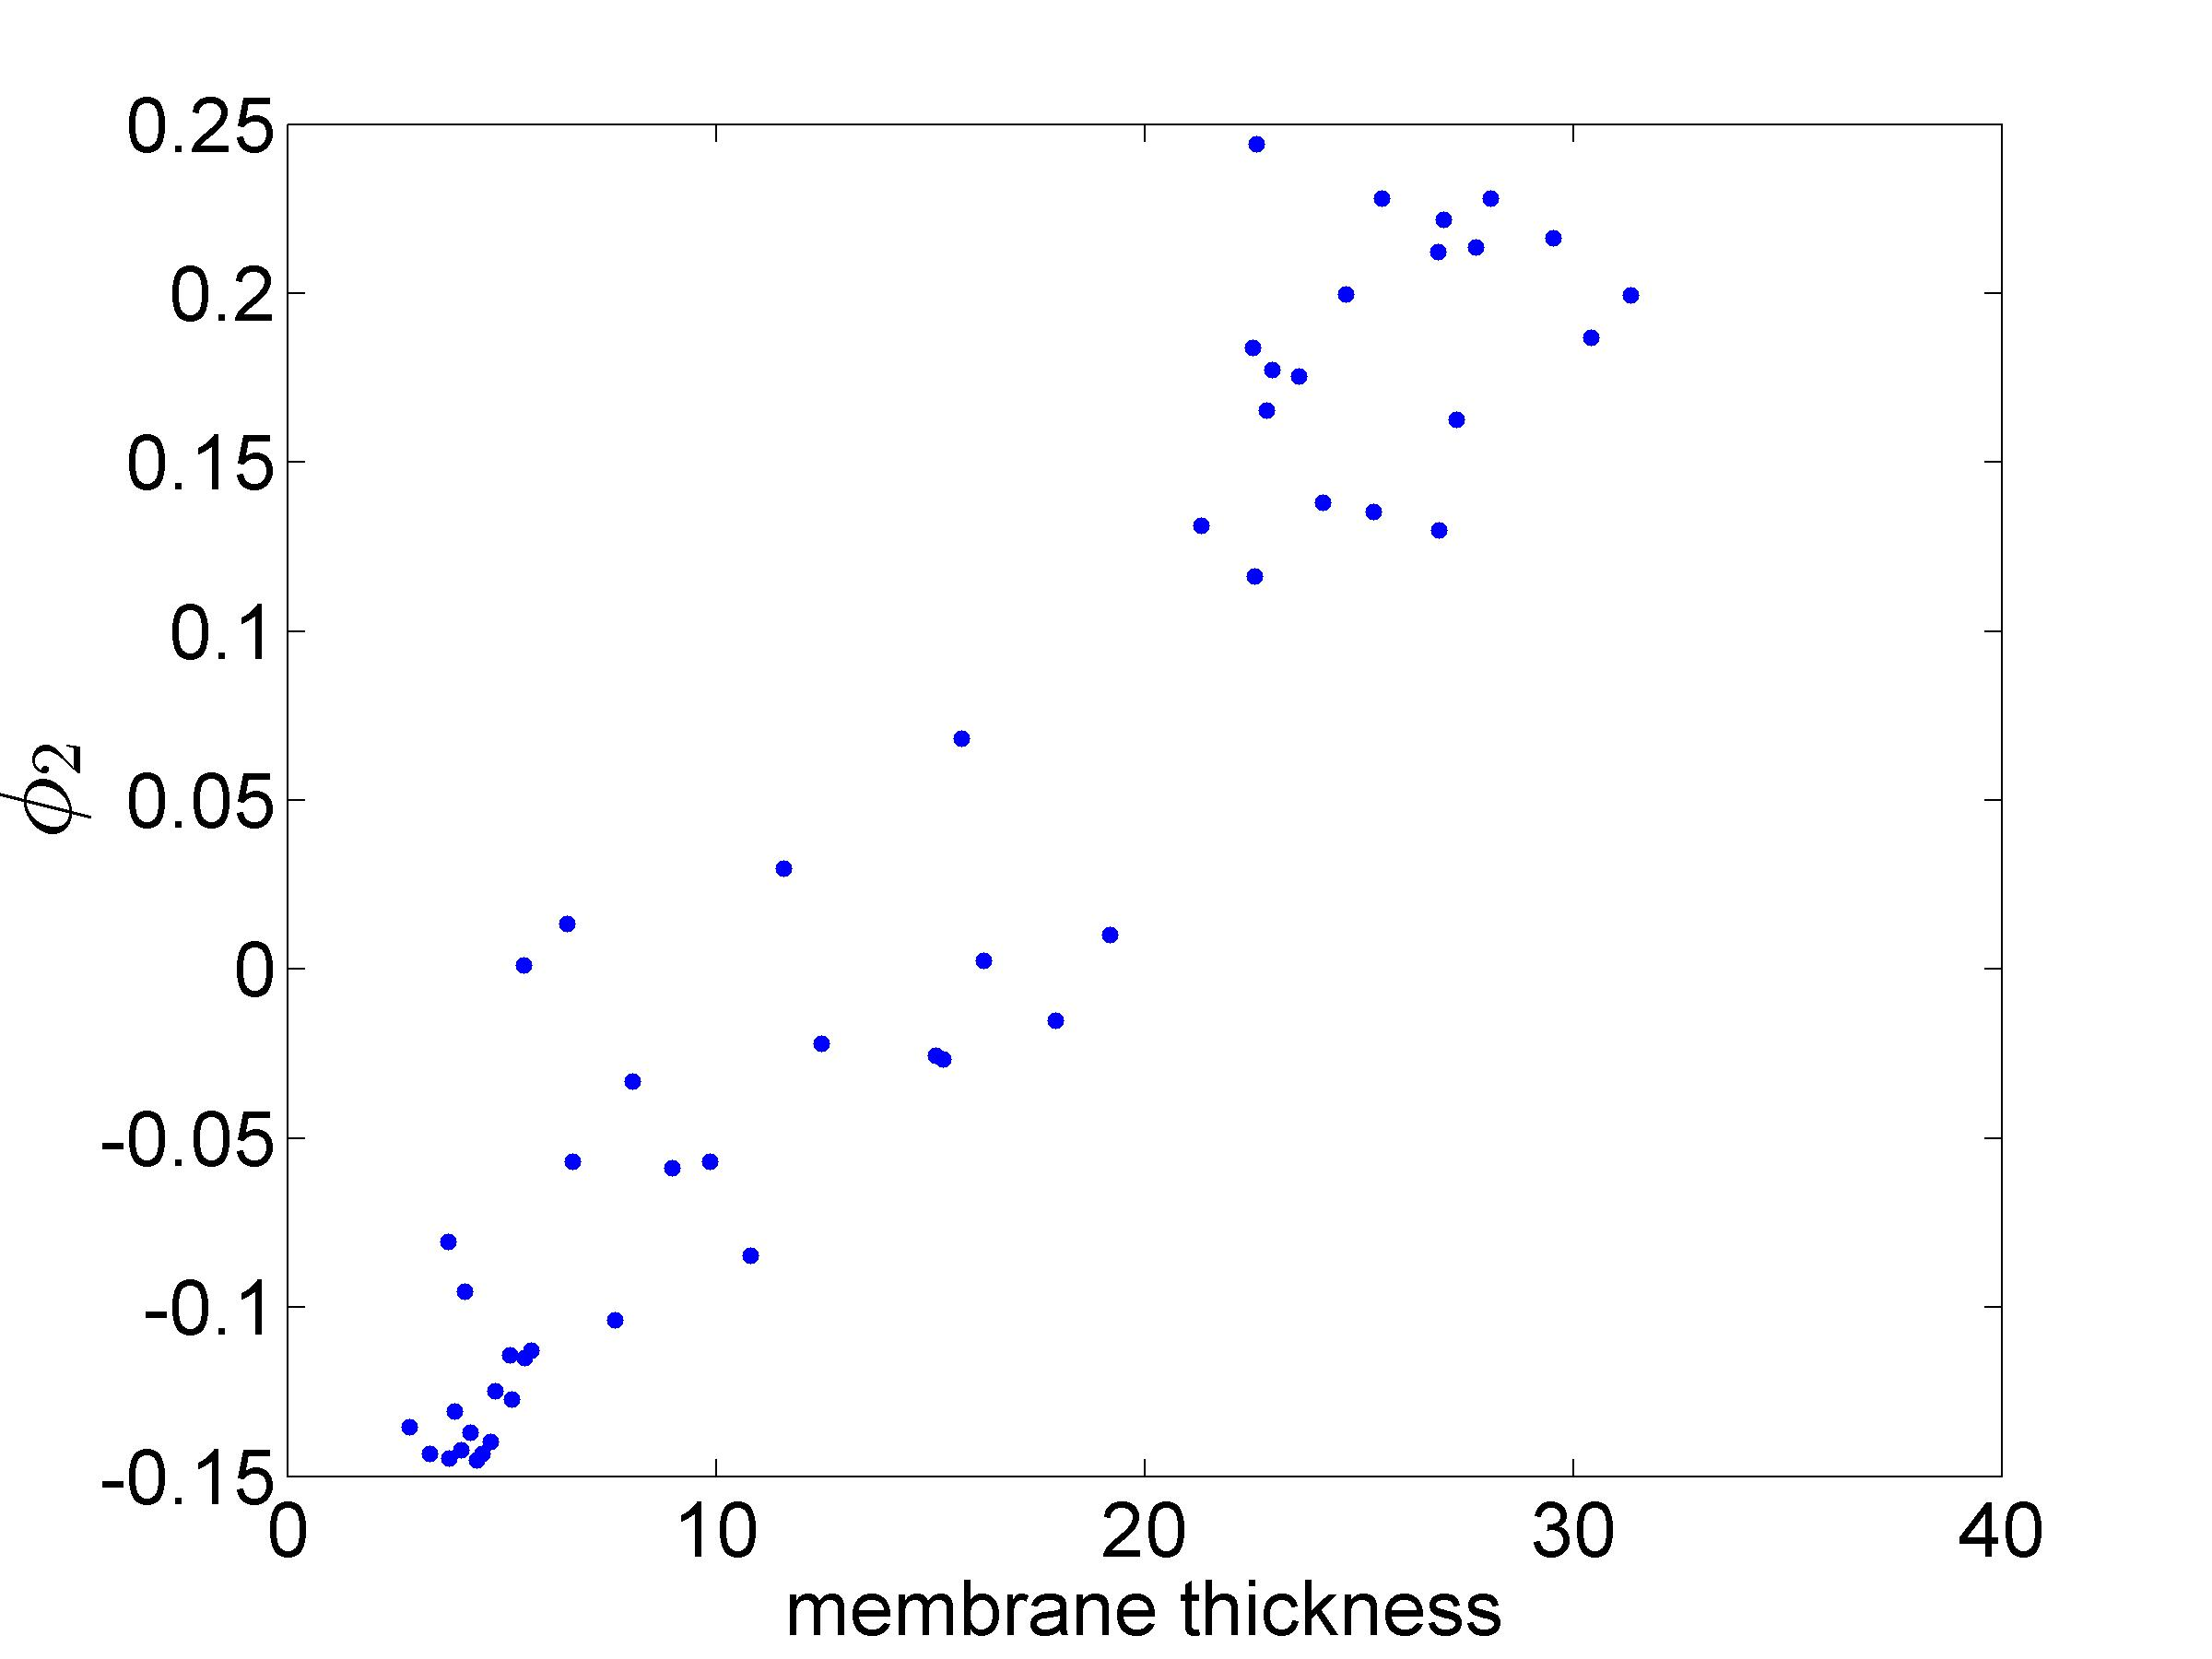
\includegraphics[width=0.3\textwidth]{DMAPS_time_corr}	
	
	\centering
  \begin{tikzpicture}
  	\node (unordered) {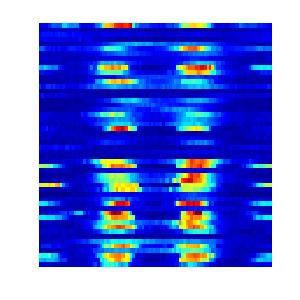
\includegraphics[width=0.3\textwidth]{data_unordered}};
  	\node[right of=unordered, node distance=0.5\textwidth] (ordered) {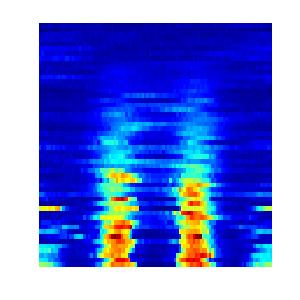
\includegraphics[width=0.3\textwidth]{data_ordered_DMAPS}};
    \draw [->] (unordered.east) -- (ordered.west);    
  \end{tikzpicture}
  
  There is a significantly better grouping of the secondary peaks when using DMAPS.
\end{frame}